\documentclass[12pt]{beamer}

\input{inc.tex}

\usepackage{mathrsfs}
\usetikzlibrary{positioning}
\usepackage{tikz-cd}
\usepackage{ebproof}
\newcommand\M{\text{M}(X\uplus X^{-1})}
\newcommand\G{\mathscr{G}(X)}
\renewcommand\F{\mathscr{F}(X)}
\newcommand\V{\mathbb{V}}
\newcommand\E{\mathbb{E}}
\newcommand\D{\mathbb{D}}
\newcommand\bet{\rightarrow_\beta}
\newcommand\beq{=_\beta}
\newcommand\Rel{\text{Rel}}
\newcommand\Set{\text{Set}}
\newcommand\Oper{\text{Oper}}
\newcommand\Inv{\text{Inv}}
\newcommand\Pol{\text{Pol}}
\renewcommand\P{\mathscr{P}}
\newcommand\ar{\text{ar}}
\newcommand\arf{\text{ar}}
\newcommand\csp{\text{CSP}}
\renewcommand\C{\mathscr{C}}
\newcommand\fset{\text{FinSet}}
\newcommand\ffun{\text{FinFun}}
\newcommand\im{\text{Im }}
\newcommand\sem[1]{\llbracket {#1} \rrbracket}
\newcommand\ext{\text{Ext}}
\newcommand\fns{\mathscr{F}}
\newcommand\brk[1]{[ {#1} ]}
\newcommand\psh{\text{PSh}}
\newcommand\sh{\text{Sh}}
\newcommand\shc{\text{Sh}_\text{can}}
\newcommand{\tproof}[1]{{\scantokens{\begin{prooftree}#1\end{prooftree}}}}
\newcommand{\cf}{\mathbb{F}}
\newcommand{\tsigma}{\widetilde{\Sigma}}
\newcommand{\tgamma}{\widetilde{\Gamma}}
\newcommand{\tlambda}{\widetilde{\Lambda}}
\newcommand{\colim}{\text{colim}}
\newcommand{\fcsp}{\text{FCSP}}
\newcommand{\op}{\text{op}}
\newcommand{\tf}{\widetilde{F}}
\newcommand{\tg}{\widetilde{G}}
\newcommand{\tH}{\widetilde{H}}
\newcommand{\ml}[1]{\langle{#1}\rangle}


%  ____                                    ____             __ _       
% | __ )  ___  __ _ _ __ ___   ___ _ __   / ___|___  _ __  / _(_) __ _ 
% |  _ \ / _ \/ _` | '_ ` _ \ / _ \ '__| | |   / _ \| '_ \| |_| |/ _` |
% | |_) |  __/ (_| | | | | | |  __/ |    | |__| (_) | | | |  _| | (_| |
% |____/ \___|\__,_|_| |_| |_|\___|_|     \____\___/|_| |_|_| |_|\__, |
%                                                                |___/ 
\usepackage{etoolbox}
\makeatletter
\preto{\@verbatim}{\topsep=0pt \partopsep=0pt }
\makeatother

% Le logo
\logo{\includegraphics[scale=0.07]{logo.png}}

% Au début de chaque section
\AtBeginSection[]{
	\begin{frame}
		\frametitle{\textbf{\insertsectionhead}}
		\framesubtitle{Partie \thesection}
		\tableofcontents[currentsection,hideothersubsections]
	\end{frame}
}

% Au début de chaque sous-section
\AtBeginSubsection[]{
	\begin{frame}
		\frametitle{\textbf{Partie} \thesection-\thesubsection}
		\begin{block}{Sous-partie \thesubsection}
			\Large \textbf{\insertsubsectionhead}
		\end{block}
	\end{frame}
}

%Put a nice theme
\usetheme{Berkeley}
\beamertemplatenavigationsymbolsempty
\makeatletter
\g@addto@macro\scriptsize{%
\setlength\abovedisplayskip{1pt}
\setlength\belowdisplayskip{1pt}
\setlength\abovedisplayshortskip{1pt}
\setlength\belowdisplayshortskip{1pt}
}
\g@addto@macro\normalsize{%
\setlength\abovedisplayskip{1pt}
\setlength\belowdisplayskip{1pt}
\setlength\abovedisplayshortskip{1pt}
\setlength\belowdisplayshortskip{1pt}
}
\makeatother
\setbeamertemplate{itemize item}[square]
\setbeamertemplate{itemize subitem}[triangle]

%  ____                                        _   
% |  _ \  ___   ___ _   _ _ __ ___   ___ _ __ | |_ 
% | | | |/ _ \ / __| | | | '_ ` _ \ / _ \ '_ \| __|
% | |_| | (_) | (__| |_| | | | | | |  __/ | | | |_ 
% |____/ \___/ \___|\__,_|_| |_| |_|\___|_| |_|\__|
%                                                  
\author{Luc Chabassier\and Simon Cabuche}
\title[CSP catégoriques]
    {Une approche catégorique aux problèmes CSP\\
        {\normalsize Mémoire de L3}}
\institute{\begin{center}École Normale Supérieure\\
    DMA
\end{center}}
\date{\small Sous la direction de Damiano Mazza}


\begin{document}
\addtobeamertemplate{block begin}{\setlength\abovedisplayskip{0pt}}

\begin{frame}
    \maketitle
\end{frame}

\begin{frame}
    \tableofcontents
\end{frame}

\section[CSP]{Problèmes de satisfaction de contraintes}

\subsection{Définitions générales}

\begin{frame}
    \frametitle{Définition}

    \begin{block}{Logique régulière}
        \[\begin{array}{rcl}
        P,Q & := & R_1(x_1, \dots, x_{\alpha_1}) \\
        & |  & \vdots                        \\
        & |  & R_n(x_1, \dots, x_{\alpha_n}) \\
        & |  & P \wedge Q                    \\
        & |  & \exists x \ P                  \\
        & |  & \top                          \\
        \end{array}\]
    \end{block}
    \pause
    \begin{block}{CSP}
        A un CSP est associé un problème $\csp (D,\Sigma)$, dont une instance est la
        donnée d'une formule $P$ de la logique régulière sur $\Sigma$, et il s'agit de
        savoir si $D \models P$.
    \end{block}
\end{frame}

\begin{frame}
    \frametitle{Exemple des CSP}

    \begin{exampleblock}{$k$-SAT pour $k\geq 2$}
        $$\Sigma_{k-SAT} = \{R_{a_1,\dots,a_k}|(a_1,\dots,a_k) \in \{0,1\}^k\}$$\\ Et
        pour $(a_1,\dots,a_k) \in \{0,1\}^k$~: $$r_{a_1,\dots,a_k} = \{0,1\}^k -
        \{a_1,\dots,a_k\} $$
    \end{exampleblock}
    \pause
    \begin{alertblock}{Remarque}
        On a donc des problèmes polynomiaux ($2$-SAT) et des problèmes $NP$-complets
        ($3$-SAT) dans les CSP.
    \end{alertblock}
\end{frame}

\begin{frame}
    \frametitle{Résultat principal}

    \begin{block}{Conjecture de Feder et Vardi, 1998}
        Tout problème CSP est soit polynomial, soit $NP$-complet.
    \end{block}
    \pause
    \begin{alertblock}{TODO noms des auteurs qui ont prouvé la conjecture, 2017}
        Cette conjecture est prouvée !
    \end{alertblock}
\end{frame}

\subsection{Hiérarchisation}

\begin{frame}
    \frametitle{Réduction}

    \begin{block}{Définition}
        Soient $(D,\mathcal{D})$ et $(E,\mathcal{E})$ deux CSP. On dit que
        $(D,\mathcal{D})$ se réduit à  $(E,\mathcal{E})$ s'il existe une réduction
        LogSPACE du problème $CSP(D,\mathcal{D})$ au problème $CSP(E,\mathcal{E})$,

        On notera $(D,\mathcal{D}) \leq (E,\mathcal{E})$
    \end{block}
    \pause
    \begin{exampleblock}{Lemme}
        L'ensemble des CSP munit de la réduction est un préordre.
    \end{exampleblock}
\end{frame}

\begin{frame}
    \frametitle{pp-définissabilité}

    Soient $(D,\mathcal{D})$ et $(D,\mathcal{E})$ deux CSP sur le même domaine $D$.

    \begin{block}{Définition}
        On dit que $(D,\mathcal{D})$ pp-définit
        $(D,\mathcal{E})$ lorsque chaque relation dans $\mathcal{E}$ peut être
        définie par une formule régulière du premier ordre qui n'utilise que
        des relations de $\mathcal{D}$.
    \end{block}
    \pause
    \begin{exampleblock}{Proposition}
        Si $(D,\mathcal{D})$ pp-définit $(D,\mathcal{E})$,
        alors $(D,\mathcal{E}) \leq (D,\mathcal{D})$.
    \end{exampleblock}
\end{frame}

\begin{frame}
    \frametitle{pp-interprétabilité}

    \begin{block}{Définition}
        $(D,\mathcal{D})$
        pp-interprète $(E,\mathcal{E})$ lorsqu'il existe $n \in \mathbb{N}$, $F
        \subset D^n$ et une application surjective $f : F \rightarrow E$ telle que
        $(D,\mathcal{D})$ pp-définit :
        \begin{itemize}
            \item la relation $F$
            \item l'image réciproque par $f$ de la relation d'égalité sur $E$
            \item l'image réciproque par $f$ de chaque relation dans $\mathcal{E}$
        \end{itemize}
    \end{block}
    \pause
    \begin{exampleblock}{Proposition}
        Si $(D,\mathcal{D})$ pp-interprète $(E,\mathcal{E})$, alors
        $(E,\mathcal{E}) \leq (D,\mathcal{D})$.
    \end{exampleblock}
\end{frame}

\subsection{Catégorie $\csp$}

\begin{frame}
    \frametitle{Définition}
    \begin{itemize}[<+->]
        \item Les objets sont les éléments de $CSP(\star)$ : il s'agit des couples
            $(D,\mathcal{D})$ avec $D$ un ensemble fini et $\mathcal{D}$ un
            ensemble fini de relations sur $D$.
        \item Les morphismes entre  $(D,\mathcal{D})$ et  $(E,\mathcal{E})$ sont
            des triplés $(n,F,f)$ avec $n \in \mathbb{N}$, $F \subset D^n$ et $f :
            F \rightarrow E$ une application surjective telle que les images
            réciproques par $f$ des relations de $\mathcal{E}$, de la relation
            d'égalité sur $E$, et $F$ soient pp-définissables dans
            $(D,\mathcal{D})$.
    \end{itemize}
\end{frame}


\section[Catégorie]{Une catégorie pour les CSP}

\subsection{Construction}

\begin{frame}
    \frametitle{Motivation}
    \begin{block}{Sémantique selon un faisceau}
        \[\sem{\phi}_F := \{(F\pi_1(x), \dots F\pi_n(x)) | x\in F\phi\}\]
    \end{block}
    \pause
    \begin{block}{CSP du faisceau}
        \[\csp_F := (F\star, \{\sem{R(x_1,\dots, x_k)}_F,\dots\})\]
    \end{block}
    \pause
    \begin{exampleblock}{Résultat voulu}
        \[\sem{\phi}_{\csp_F} = \sem{\phi}_F\]
    \end{exampleblock}
\end{frame}

\begin{frame}
    \frametitle{Intuition}

    \begin{block}{Nouvelle vision de l'alphabet}
        \[\begin{tikzcd}[ampersand replacement=\&, row sep=small]
            \& \star \arrow[ddl, shift right, swap, "f_1^1"]
                    \arrow[ddl]
                    \arrow[ddl, shift left, "f_{\text{ar}(R_1)}^1"]
                    \arrow[ddr, shift right, swap, "f_1^m"]
                    \arrow[ddr]
                    \arrow[ddr, shift left, "f_{\text{ar}(R_m)}^m"]
                    \\
            \& \& \\
            R_1 \& \dots \& R_m \\
        \end{tikzcd}\]
    \end{block}
    \visible<2->{
    \begin{block}{Interprétation en formule}
        \only<2>{Analogie avec les graphes~:
        \[\begin{tikzcd}[ampersand replacement=\&]
            v \arrow[r, bend right, "s"] \arrow[r, bend left, "t"] \& e \\
        \end{tikzcd}\]}
        \only<3>{
        \[\bigwedge_{1\leq i\leq m} \bigwedge_{x\in AR_i}
                R_i(Af_1^i(x), \dots Af_{\ar(R_i)}^i(x)) \]
        }
    \end{block}}
\end{frame}

\begin{frame}
    \frametitle{Résultat fondamental}

    Soient~:\begin{itemize}
        \item $Y : \psh(\C)\rightarrow\shc(\psh(\C))$ le plongement de Yoneda sur
            $\psh(\C)$.
        \item $y : \C\rightarrow\psh(\C)$ le plongement de Yoneda sur $\C$.
        \item \[L = \left\{\begin{array}{ccc}
                 \shc(\psh(\C)) & \rightarrow & \psh(\C) \\
                 F              & \mapsto     & F\circ y^\text{op} \\
            \end{array}\right.\]
    \end{itemize}

    Alors $Y$ est une équivalence de catégories d'inverse $L$.
    \pause

    \begin{exampleblock}{Notation}
        On note alors $\C_\Sigma = \psh(\Sigma)$ muni de sa topologie canonique.
    \end{exampleblock}
\end{frame}

\subsection{Résultats}

\begin{frame}
    \frametitle{Nouvelle représentation d'une formule}

    \begin{block}{Séquent associé à une formule}\label{formSeq}
        Soit $\phi$ une formule conjonctive que l'on suppose mise sous la
        forme canonique $\exists x_1,\dots\exists x_n, R(\dots)\wedge R(\dots)$.
        
        On y associe le séquent~:
        \[\ml{\phi} = x_1,\dots x_n\vdash R(\dots), \dots, R(\dots)\]
    \end{block}
    \pause
    \begin{exampleblock}{Colimites usuelles}\begin{itemize}[<+->]
        \item $\ml{\mathbf{0}} = x\vdash$
        \item Si $\ml{\phi} = \Xi\vdash\Delta$ et $\ml{\phi'} = \Xi'\vdash\Delta'$,
            alors $\ml{\phi\times\phi'} = \Xi,\Xi'\vdash\Delta,\Delta'$
        \item $\ml{n\ast} = x_1,\dots,x_n\vdash$
    \end{itemize}\end{exampleblock}
\end{frame}

\begin{frame}
    \frametitle{Correction}

    Soit $F\in\shc{\C_\Sigma}$ et $X\in\psh{\Sigma}$.

    \begin{exampleblock}{Proposition}
        \[\sem{\phi}_{\csp_{LF}} = \sem{\phi}_F\]
        \pause
        \[\sem{\phi}_{\csp_X} = \sem{\phi}_{YX}\]
    \end{exampleblock}
\end{frame}

\section[pp-interprétabilité]{PP-interprétabilité catégorique}

\subsection{Comma-catégories à la rescousse}

\begin{frame}
    \frametitle{Motivation}

    \begin{alertblock}{Problème}
        Pas de distinction possibles entre variables libres et variables liées~!
    \end{alertblock}
    \pause
    \begin{block}{Approche naïve}
        On prend un couple $(f,\phi)$ où $f$ est une fonction de $n$ vers $\phi\star$.
    \end{block}
    \pause
    \begin{exampleblock}{Remarque}
        C'est équivalent à prendre une flèche dans $\C_\Sigma$ de $n\ast$ vers $\phi$.
    \end{exampleblock}
\end{frame}

\begin{frame}
    \frametitle{Définitions}

    \begin{block}{Définition : $\cf$}
        On note $\cf$ la catégorie squelette de $\fset$.
    \end{block}
    \pause
    \begin{block}{Définition : $\ffun$}
        On note $\ffun := \fset^\mathbf{2}$ la catégorie des flèches de $\fset$.
    \end{block}
    \pause
    \begin{block}{Définition : foncteur $\arf$}
        \[\arf : \left\{\begin{array}{ccc}
            \cf & \rightarrow & \C_\Sigma \\
            n   & \mapsto     & n\ast \\
        \end{array}\right.\]
    \end{block}
\end{frame}

\begin{frame}
    \frametitle{Définition}

    \begin{block}{Catégorie des formules avec variables liées}
        On définit $\tsigma := \arf/\C_\Sigma$.

        On dispose de deux foncteurs d'oubli canoniques~:\begin{itemize}
            \item $U_1 : \tsigma\rightarrow\cf$
            \item $U_2 : \tsigma\rightarrow\C_\Sigma$
        \end{itemize}
    \end{block}
    \pause
    \begin{exampleblock}{Proposition}
        $\tsigma$ est cocomplète.
    \end{exampleblock}
\end{frame}

\begin{frame}
    \frametitle{Injection de $\C_\Sigma$ dans $\tsigma$}

    \begin{block}{Définition}
        On définit le foncteur $\iota:\C_\Sigma\rightarrow\tsigma$ de la façon suivante~:

        \[ \iota := \left\{\begin{array}{ccc}
            \Sigma & \rightarrow & \tsigma \\
            X      & \mapsto     & \mid X\star\mid\ast\rightarrow X \\
            \theta : X\rightarrow Y & \mapsto &
                \begin{tikzcd}[ampersand replacement=\&, row sep=small, column sep=small]
                    \mid X\star\mid\ast\arrow[d]
                                       \arrow[r, "\theta_\star"]
                        \& \mid Y\star\mid\ast\arrow[d] \\
                    X\arrow[r, "\theta"]
                        \& Y \\
                \end{tikzcd} \\
        \end{array}\right. \]
    \end{block}
    \pause
    \begin{exampleblock}{Propriétés}
        $\iota$ est plein et fidèle. Il préserve donc les colimites finies.
    \end{exampleblock}
\end{frame}

\begin{frame}
    \frametitle{Adjonction entre $\cf$ et $\tsigma$}

    \begin{exampleblock}{Proposition}
        On a une adjonction~:

        \[\begin{tikzcd}[ampersand replacement=\&]
            \cf\arrow[rr, bend right, swap, "\iota\circ\arf"] \& \top
                \& \tsigma\arrow[ll, bend right, swap, "U_1"] \\
        \end{tikzcd}\]
    \end{exampleblock}
    \pause
    \begin{exampleblock}{Corollaire}
        $\arf$ préserve les colimites finies.
    \end{exampleblock}
\end{frame}

\begin{frame}[fragile]
    \frametitle{Description des colimites de $\tsigma$}

    \begin{exampleblock}{Proposition}
        \begin{center}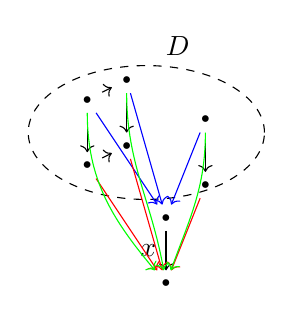
\begin{tikzpicture}[scale=0.5]
            \draw[->] (0,0)   node[above] (d1a) {\tiny$\bullet$}
                  -- (0,-1)   node[below] (d1b) {\tiny$\bullet$};
            \draw[->] (1,.5)  node[above] (d2a) {\tiny$\bullet$}
                  -- (1,-.5)  node[below] (d2b) {\tiny$\bullet$};
            \draw[->] (3,-.5) node[above] (d3a) {\tiny$\bullet$}
                  -- (3,-1.5) node[below] (d3b) {\tiny$\bullet$};
            \draw[->] (d1a) -- (d2a);
            \draw[->] (d1b) -- (d2b);
            \draw[dashed] (1.5,-0.5) ellipse (3 and 1.7);
            \draw (2.3,1.2) node[above] {$D$};

            \draw[->] (2,-3) node[above] (xa) {\tiny$\bullet$}
                  -- node[left] {$x$} (2,-4)  node[below] (xb) {\tiny$\bullet$};
            \draw[->,blue]  (d1a) -- (xa);
            \draw[->,blue]  (d2a) -- (xa);
            \draw[->,blue]  (d3a) -- (xa);
            \draw[->,red]   (d1b) -- (xb);
            \draw[->,red]   (d2b) -- (xb);
            \draw[->,red]   (d3b) -- (xb);
            \draw[->,green] (d1a) edge[out=270, in=130] (xb);
            \draw[->,green] (d2a) edge[out=270, in=100] (xb);
            \draw[->,green] (d3a) edge[out=270, in=70]  (xb);
        \end{tikzpicture}\end{center}

    \end{exampleblock}
    \pause
    \begin{exampleblock}{Corollaire}
        $U_1$ et $U_2$ préservent les colimites finies.
    \end{exampleblock}
\end{frame}

\subsection{Catégorie $\fcsp$}

\begin{frame}
    \frametitle{Portage de foncteur}

    Soit $F : \C_\Sigma^\op\rightarrow\fset$ un faisceau.

    \begin{block}{Définition}
        On définit $\tf : \tsigma^\op\rightarrow\ffun$ de la façon suivante~:
        on envoie une flèche $n\ast\rightarrow X$ sur la flèche $(F\ast)^n\leftarrow FX$.
    \end{block}
    \pause
    \begin{exampleblock}{Propriétés}
        $F$ envoie les colimites de $\C_\Sigma$ sur des limites.
        
        $\tf$ a la même propriété.
    \end{exampleblock}
\end{frame}

\begin{frame}
    \frametitle{Définition de $\fcsp$}

    \begin{itemize}[<+->]
        \item Objets~: couples $(\Sigma, F)$ où $\Sigma$ est un alphabet et
            $F\in\shc(\C_\Sigma)$ est un faisceau.

        \item Morphismes~: $(\Sigma,F)\rightarrow(\Gamma,G)$

            \[\begin{tikzcd}[ampersand replacement=\&]
                \tsigma^\op\arrow[dr, bend right, swap, "r^\op"]
                           \arrow[rr, bend left, "\tf"]
                    \& \Uparrow\theta
                    \& \ffun \\
                \& \tgamma^\op\arrow[ur, bend right, swap, "\tg"] \\
            \end{tikzcd}\]
    \end{itemize}
\end{frame}

\subsection[Foncteur $\alpha$]{Foncteur $\alpha : \fcsp\rightarrow\csp$}

\begin{frame}
    \frametitle{Définition}

    \begin{itemize}[<+->]
        \item Image d'un objet~: $\alpha(\Sigma,F) = (C,\mathcal{C})$
            où $C=F\ast$ et $\mathcal{C} := \{\sem{R_1}_F,\dots\sem{R_m}\}$.

        \item Image d'une flèche~:

            \[\begin{tikzcd}[ampersand replacement=\&]
                \tsigma^\op\arrow[dr, bend right, swap, "r^\op"]
                           \arrow[rr, bend left, "\tf"]
                    \& \Uparrow\theta
                    \& \ffun \\
                \& \tgamma^\op\arrow[ur, bend right, swap, "\tg"] \\
            \end{tikzcd}\]

            Et envoyée sur le triplet $(n,F,f)$ où $n = U_1r\iota\ast$,
            $F = \im \tg r\iota\ast$ et $f = \theta^1_{\ast|F}$.
    \end{itemize}
\end{frame}

\begin{frame}
    \frametitle{Propriété essentielle}

    Soit $r:\tsigma\rightarrow\tgamma$ qui préserve les colimites finies.

    \[\begin{tikzcd}[ampersand replacement=\&]
        \cf\arrow[dr, "\iota\circ\arf"] \& \& \& \cf \\
        \& \tsigma\arrow[r, "r"] \& \tgamma\arrow[ur, "U_1"]\arrow[dr, "U_2"] \& \\
        \C_\Sigma\arrow[ur, "\iota"] \& \& \& \C_\Sigma \\
    \end{tikzcd}\]

\end{frame}

\section{Conclusion}

\begin{frame}
    \frametitle{Travail accomplit}

    \begin{itemize}[<+->]
        \item Définition d'une catégorie représentant les CSP~: $\csp$
        \item Définition d'une catégorie représentant les CSP de
            manière fonctorielle~: $\fcsp$.
        \item Preuve d'un certains nombre de propriétés sur les objets définis.
    \end{itemize}
\end{frame}

\begin{frame}
    \frametitle{Travail restant}

    \begin{itemize}[<+->]
        \item Définir un foncteur $\gamma:\csp\rightarrow\fcsp$.
        \item Montrer qu'on a une équivalence de catégorie ou au moins adonctions
            entre $\csp$ et $\fcsp$ en utilisant $\alpha$ et $\gamma$.
        \item Prouver la dichotomie dans notre formalisme.
        \item Axiomatiser.
        \item Généraliser le résultat ?
    \end{itemize}
\end{frame}

\begin{frame}
    \frametitle{Remerciements}

    Nous tenons à remercier Damiano Mazza pour nous avoir encadré tout au long du
    mémoire et nous avoir permis d'avancer autant.
\end{frame}

\end{document}
